\section*{Figures}
\begin{figure}
  \begin{center}
  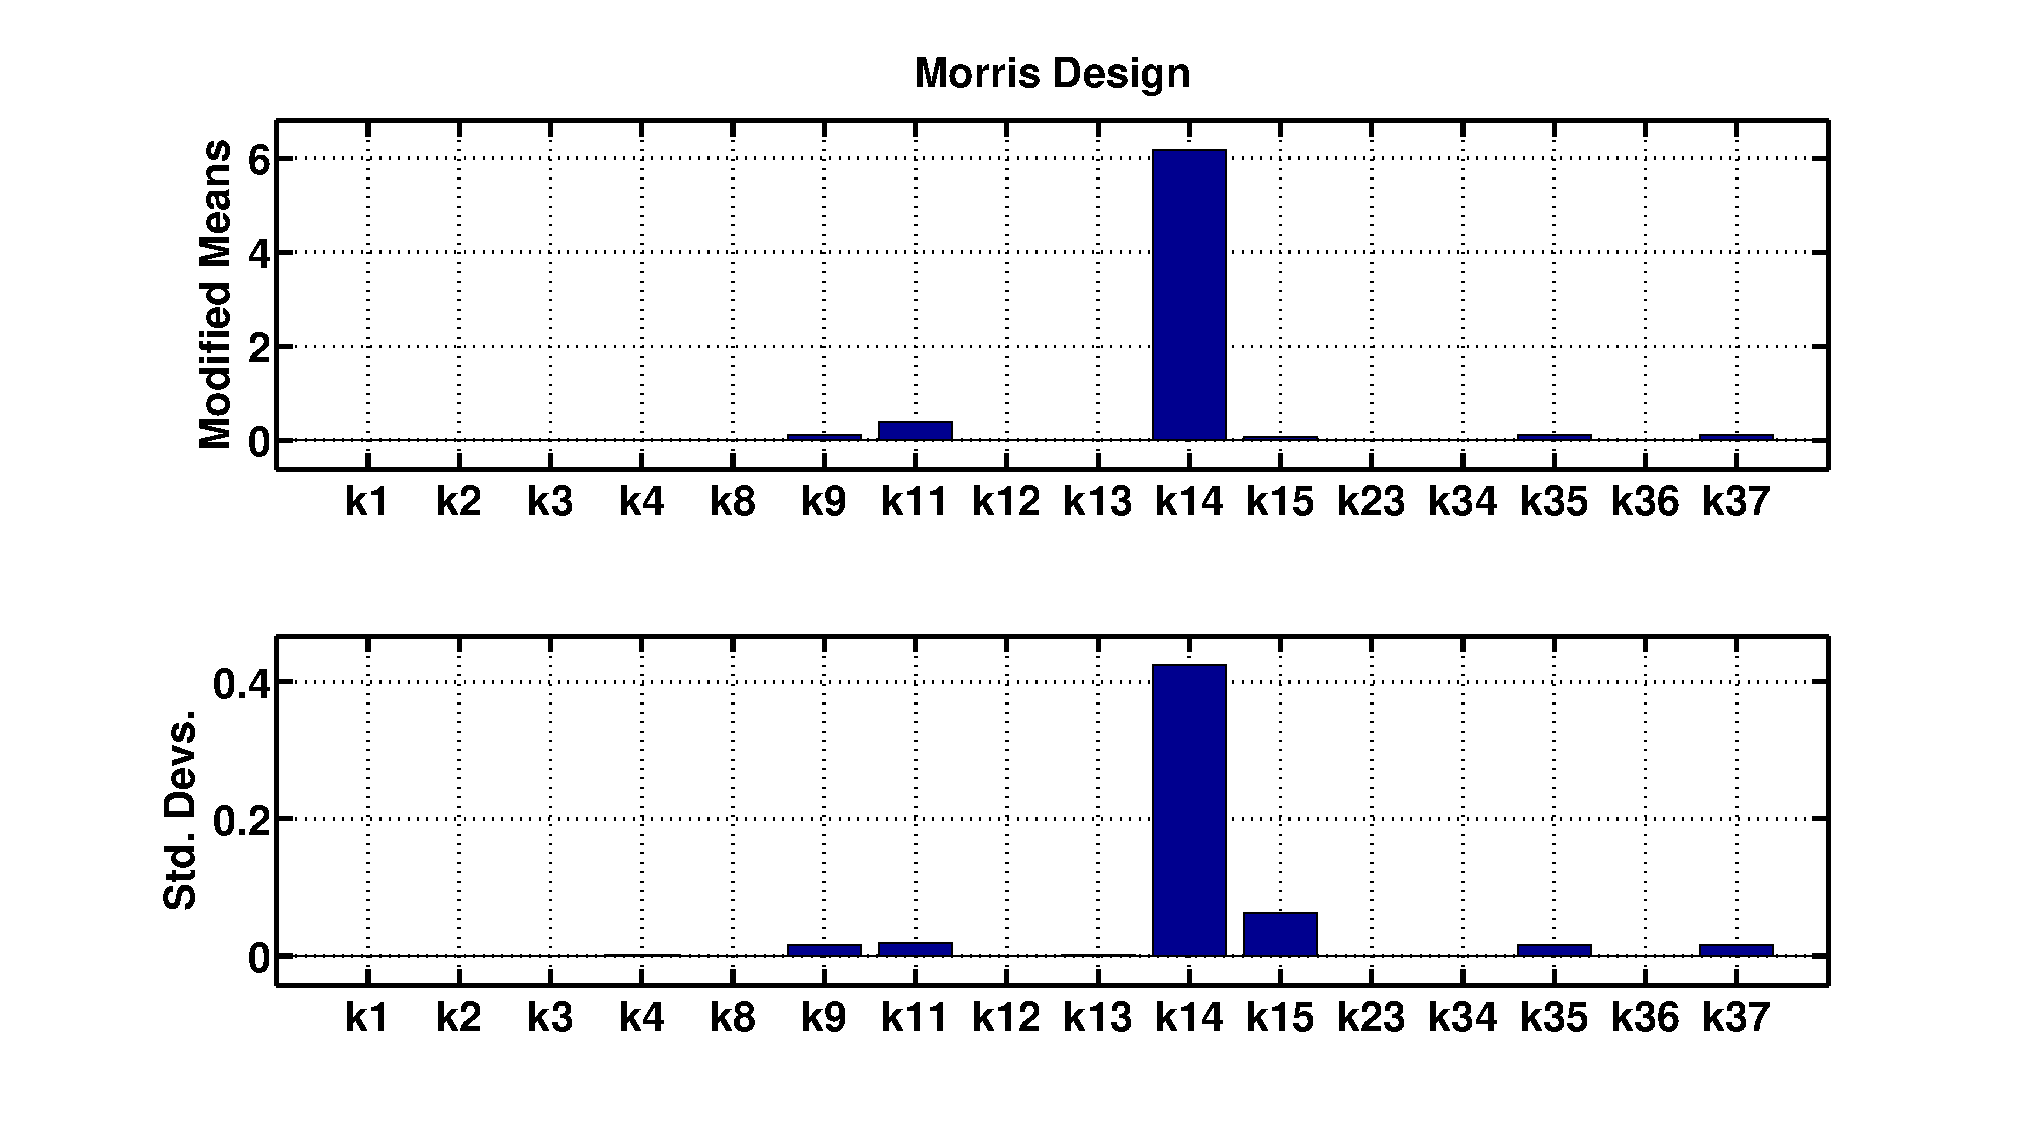
\includegraphics[width=6in]{figures/mean1.eps}
\caption{Modified means and standard deviations based sensitivity
ranking of reaction rates with respect to the total thrombin using
``Morris one at a time'' method. Horizontal axis shows reaction
rates. Vertical axis shows modified means and standard deviations
respectively. This figure indicates  that $k_{14}$ has the largest
modified mean and standard deviation,  and that $k_{14}$ is the most
sensitive to variance of total thrombin. } \label{Fig:mmean}

  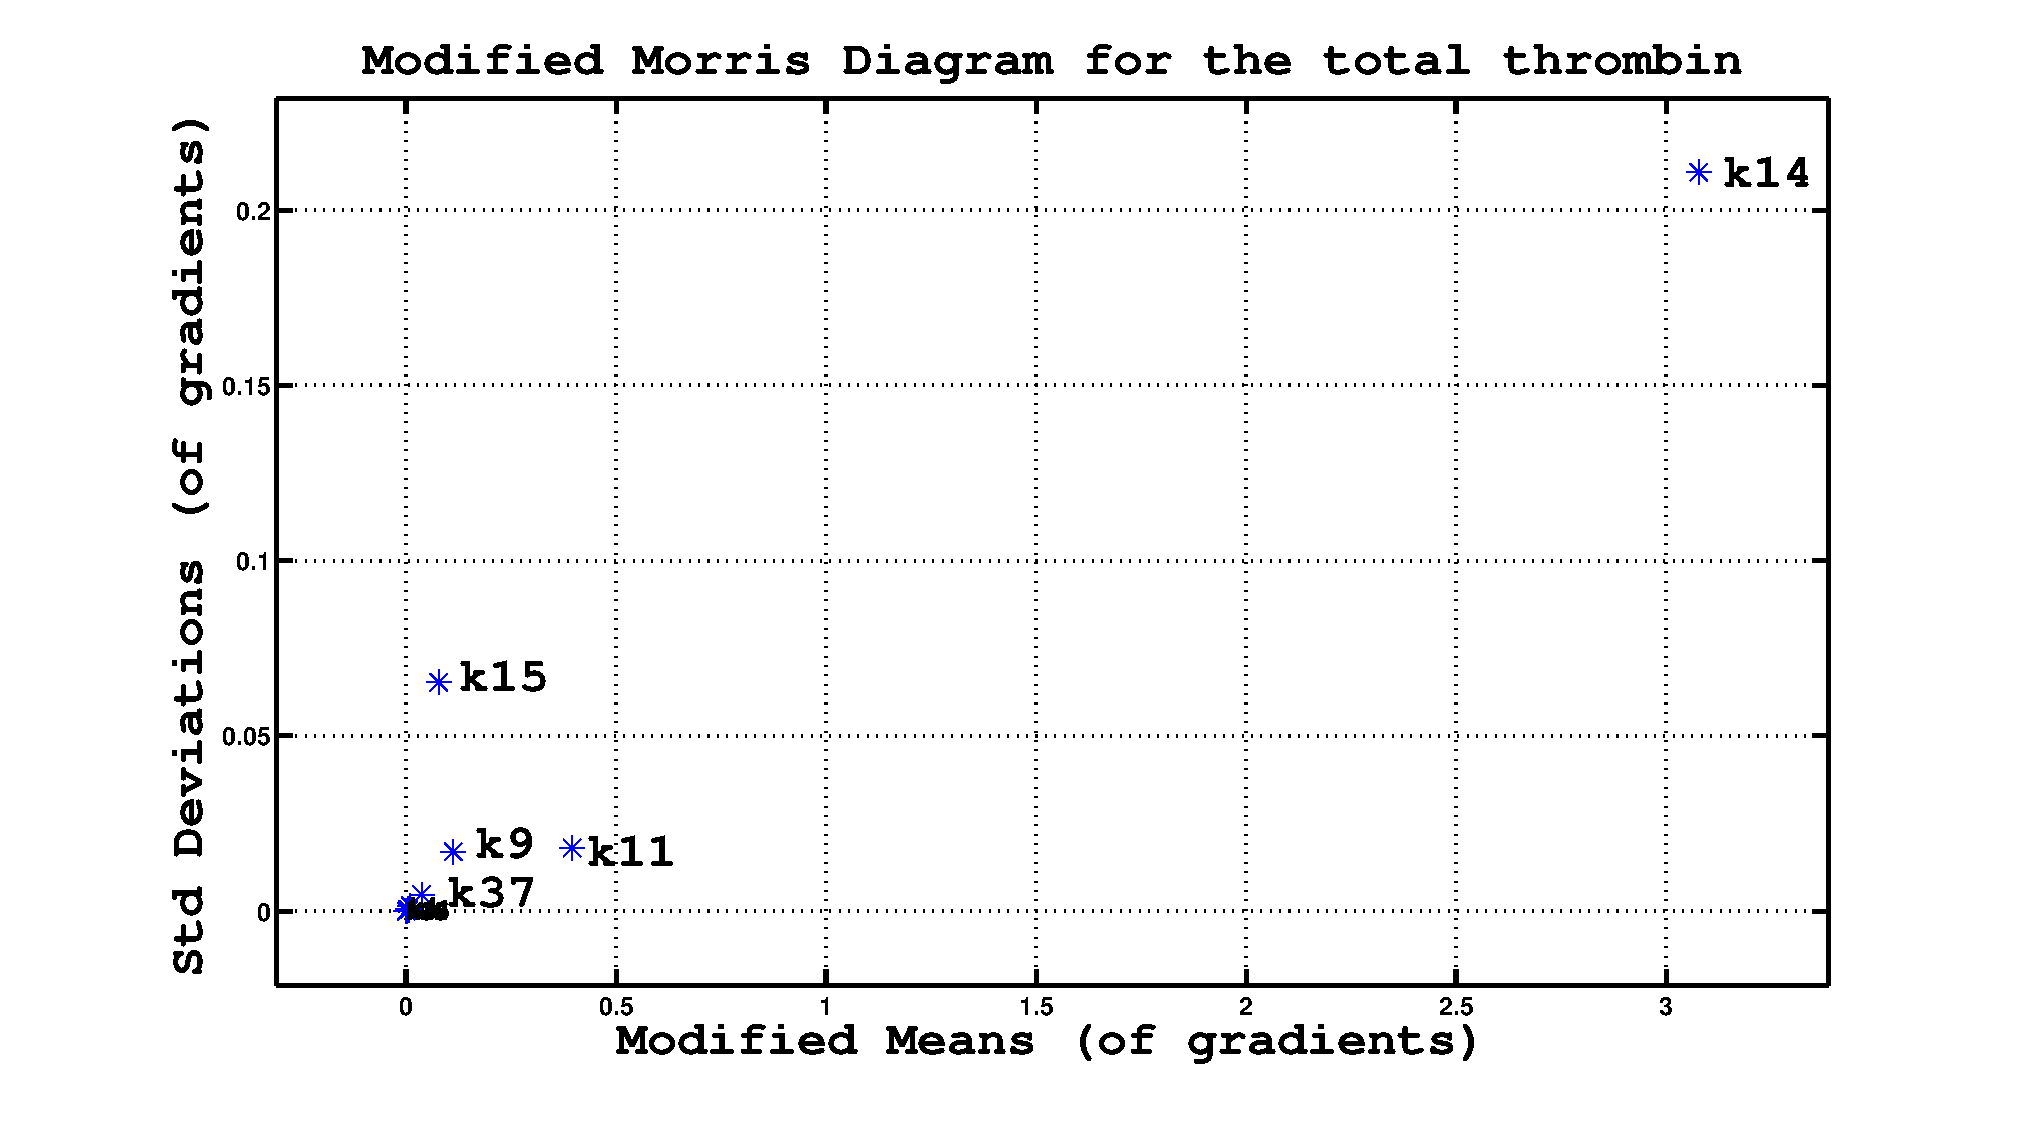
\includegraphics[width=6in]{figures/std.eps}
\caption{Modified Morris diagram on sensitivity ranking of reaction
rates with respect to the total thrombin. Ranks of sensitivity for
individual reaction rates are determined by their distance from the
origin. From this figure, the five most sensitive reaction rates are
$k_{14}$, $k_{15}$,  $k_{11}$, $k_{9}$ and $k_{37}$. The other
reaction rates cluster together due to the same magnitude of
sensitivity. } \label{Fig:std}

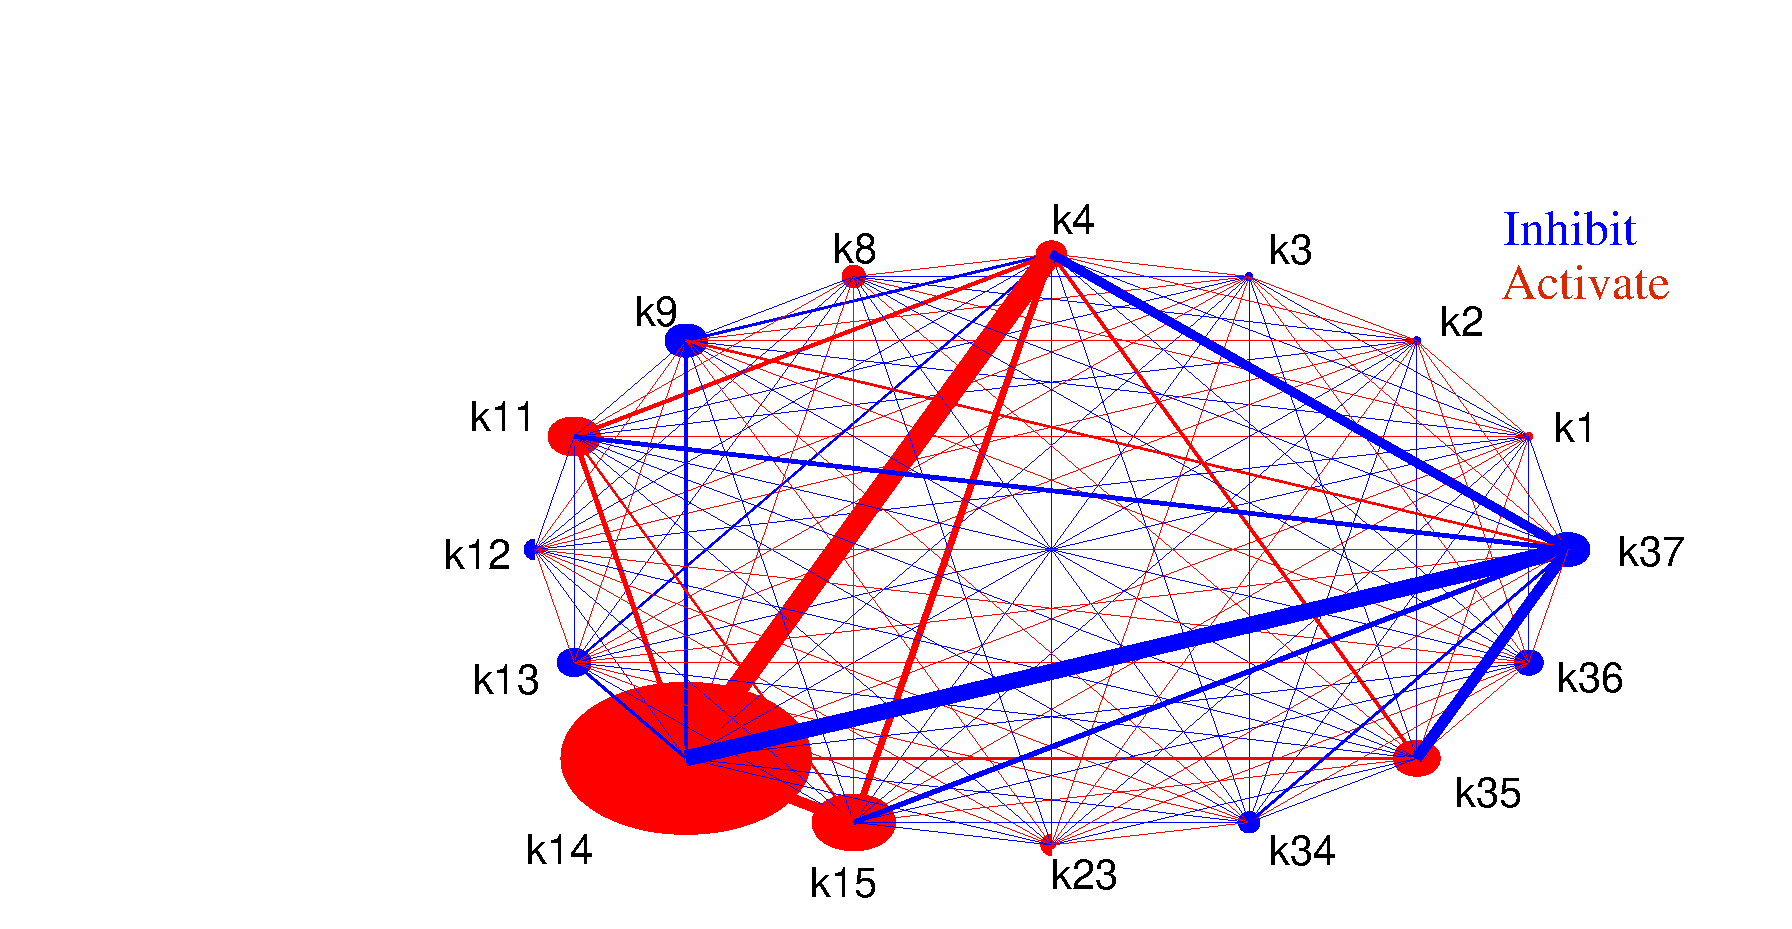
\includegraphics[width=4in,height=3in]{figures/NSA.eps}
\caption{Network graph of importance of reaction rates and the
interaction between pair reactions with respect to total thrombin.
The radius of circles corresponding to reaction rate measures the
rank of sensitivity while the width of lines of any pair of reaction
rates represents rank of their co-sensitivity. The red color
indicates that they play an activate role in generating thrombin
production while the blue color means that they inhibit the
generation of thrombin production. This figure shows that $k_{14}$,
$k_{15}$ and $k_{11}$ are the most sensitive reaction rates in
activating thrombin while $k_{37}$ and $k_{9}$ inhibit thrombin
production. Variance of $k_4$ and $k_{14}$ can play a positive role
in generation of thrombin production, however $k_{37}$ and $k_{14}$
inhibit generation of thrombin production.  } \label{fig:NSA1}

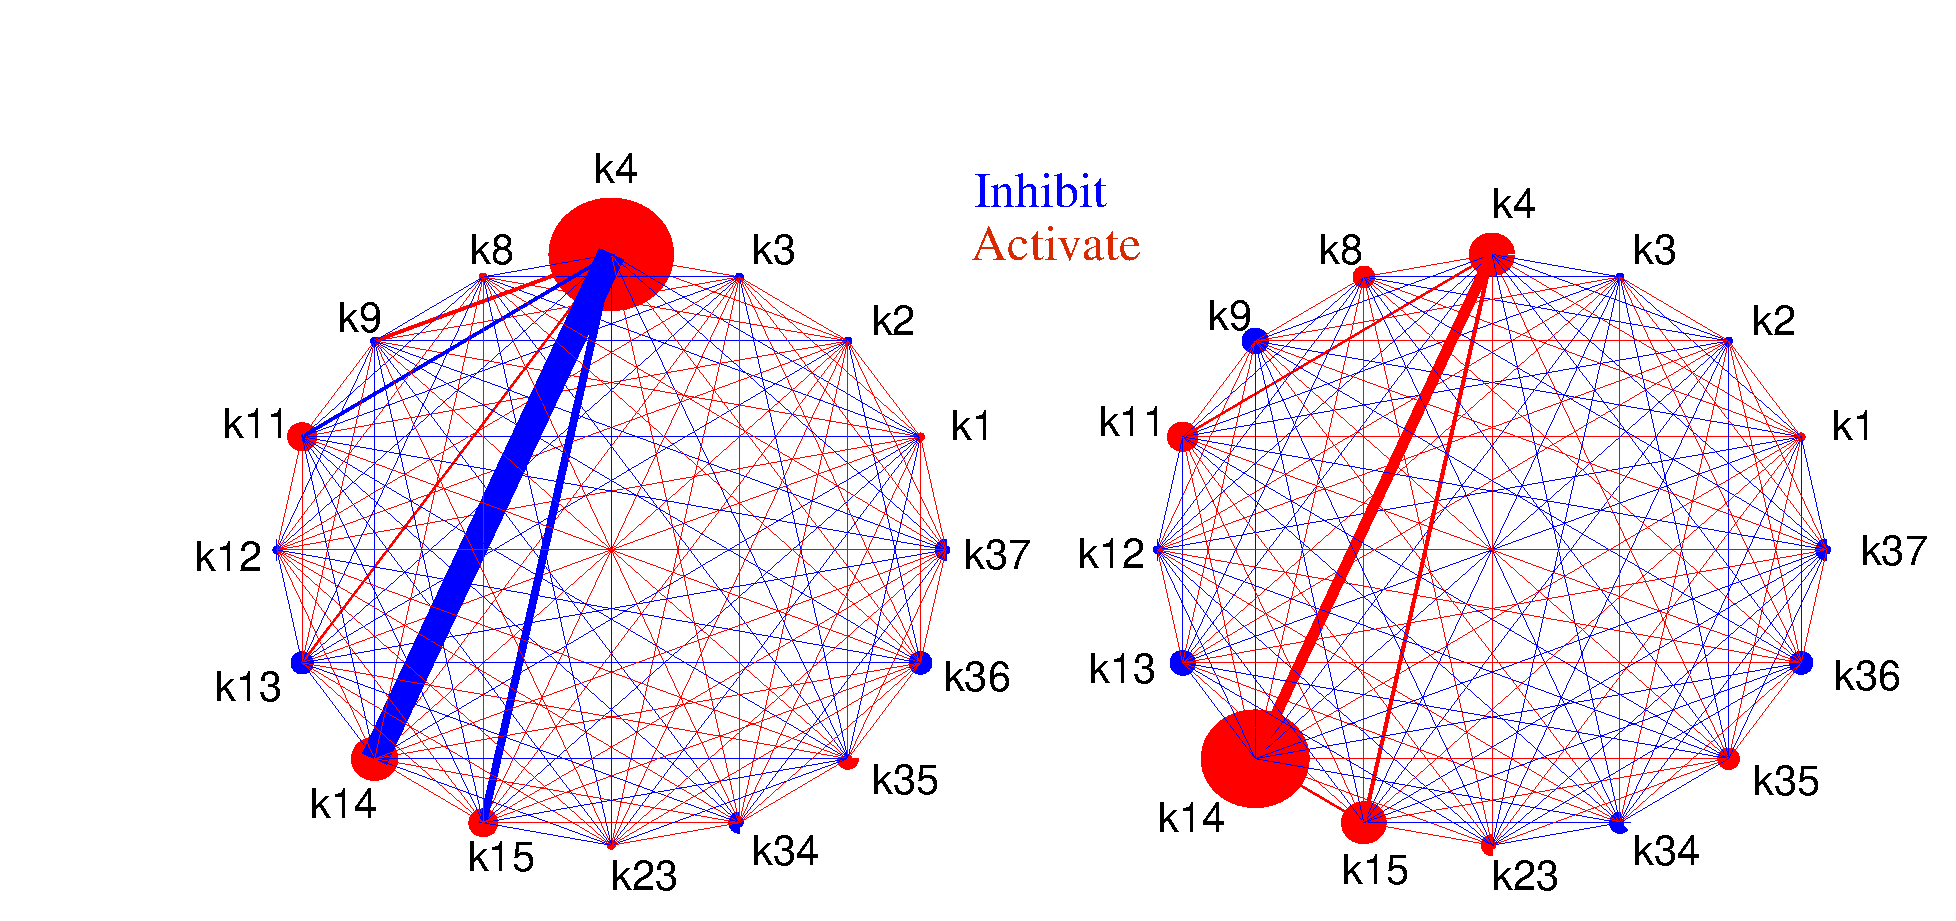
\includegraphics[width=5in,height=2.5in]{figures/nsarb33.eps}
\caption{Network graph of importance of reaction rates and the
interaction between pair reactions with respect to $x_{33}$ and
$x_{30}$ respectively. The same legend is used with Figure 3. This
figure shows that the rank of sensitivity varices with respect to
different output variables. } \label{fig:NSA}

  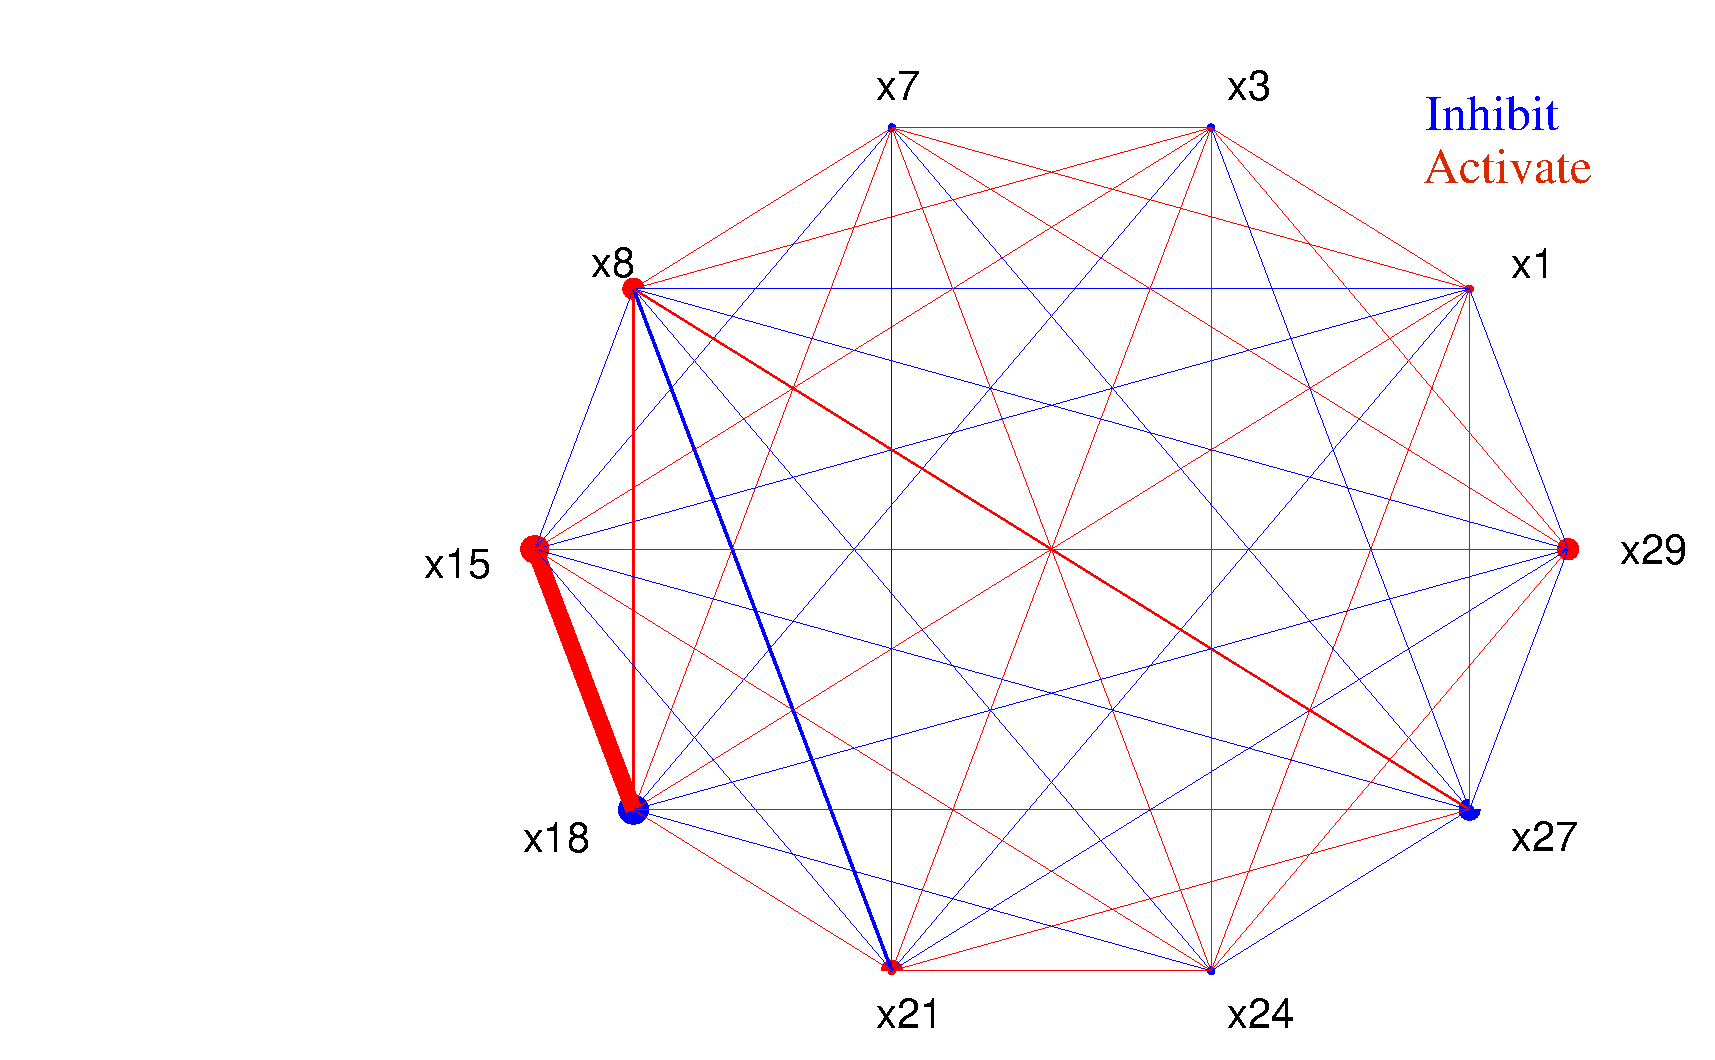
\includegraphics[width=4in]{figures/nsaic.eps}
\caption{Network graph of importance of initial condition and the
interaction between pair components with respect to total thrombin.
See the legend in Figure 3. This figure shows that factor X
($x_{15}$) is the most sensitive reaction component in activating
thrombin while TFPI ($k_{18}$) inhibits thrombin production.
Moreover, their variance can play a positive role in generation of
thrombin production.} \label{Fig:nsaic}

  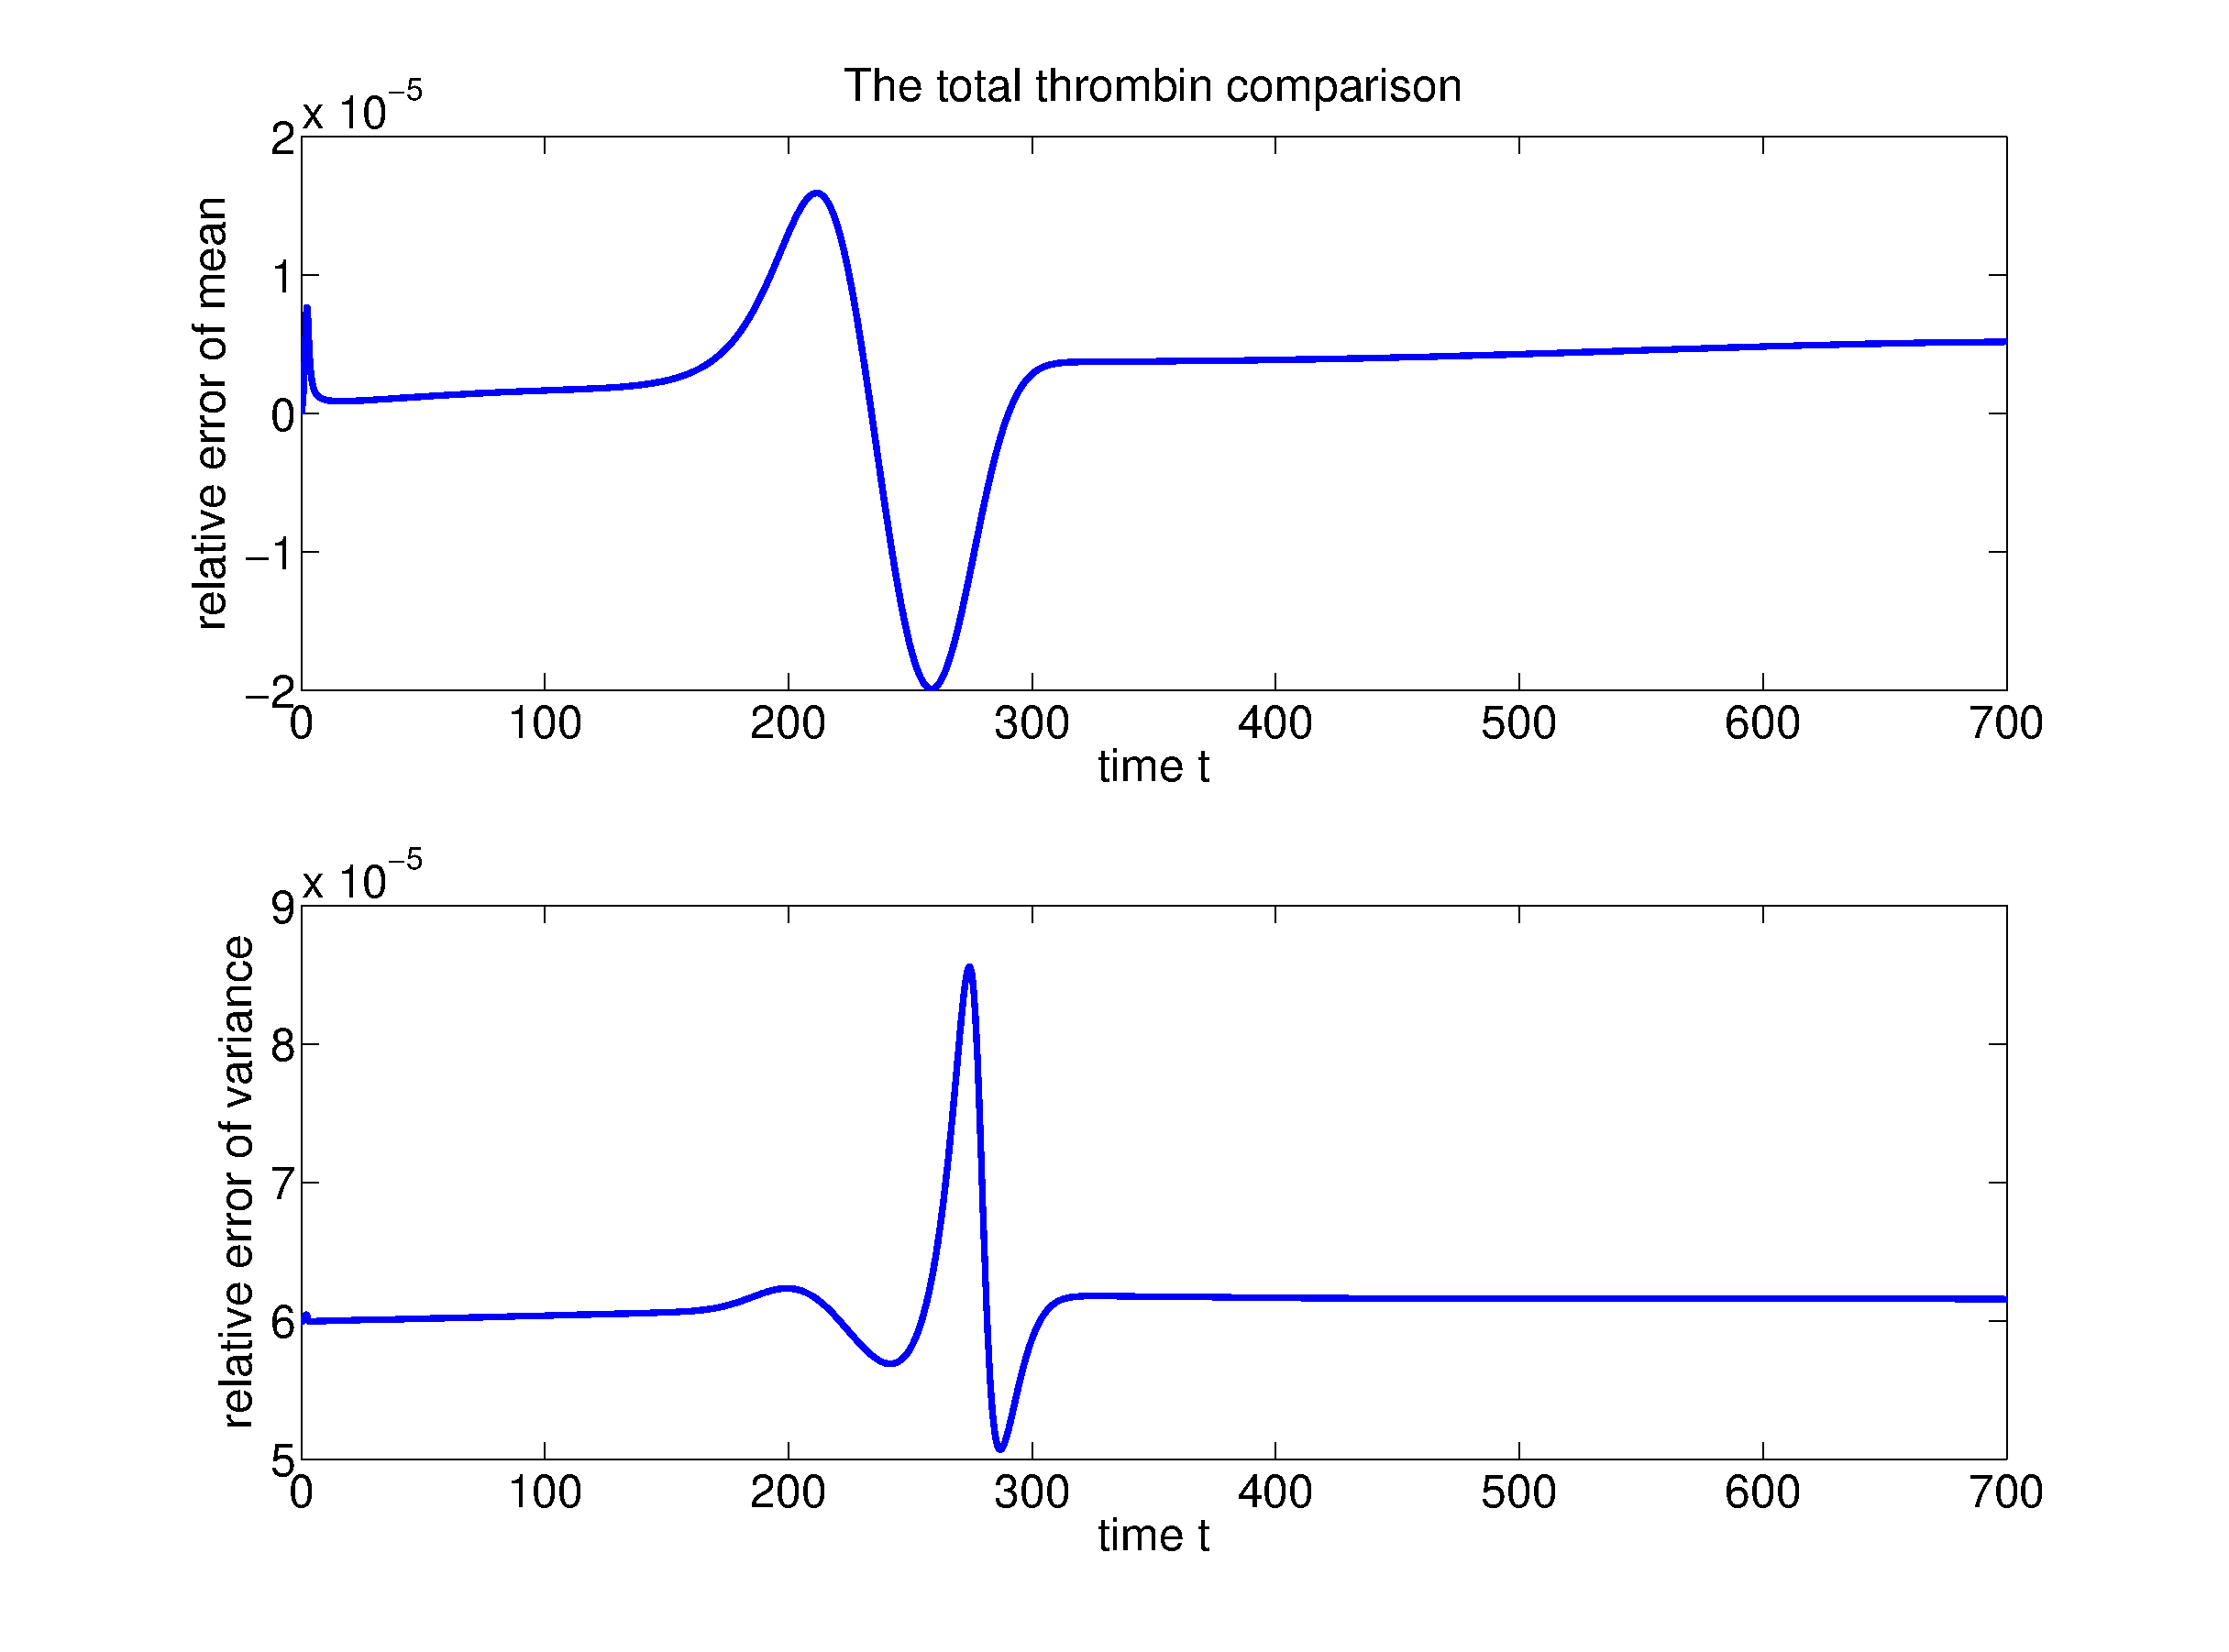
\includegraphics[width=5in]{figures/comp.eps}
\caption{The Difference of mean and variance of the total thrombin
obtained by SGPCM ($545$ points) and MC ($1000$ points). The figure
shows that the results of two methods are same under small
tolerance. %The peaks of two figures because the variance of
 %total thrombin is relatively fast at this point (See Figure 8).
 } \label{Fig:comp}

  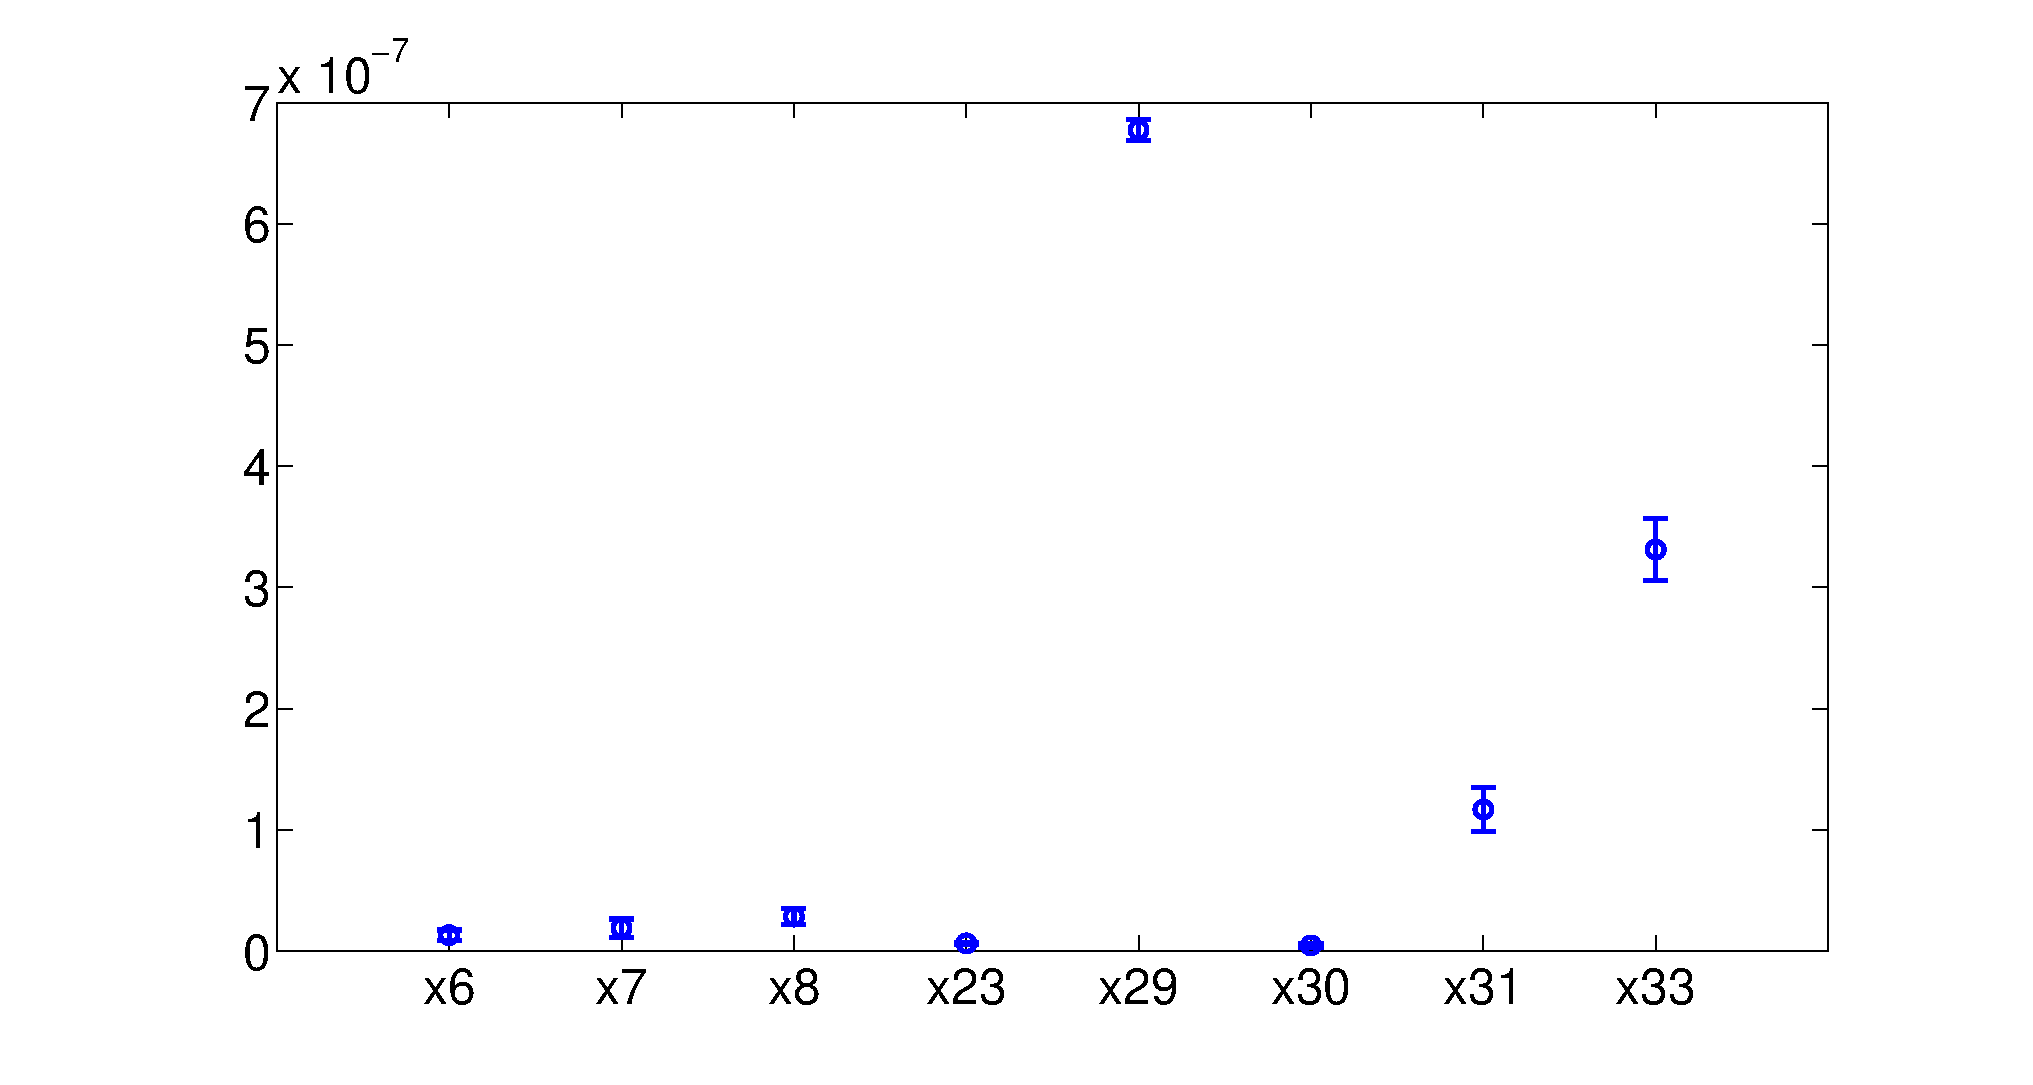
\includegraphics[width=5in]{figures/steady.eps}
\caption{Mean and error bar of steady state solutions whose
magnitude are greater than $10^{-10}$. Horizontal axis is reaction
rates. This figure shows confidence intervals of each reaction
rates.} \label{Fig:steady}

  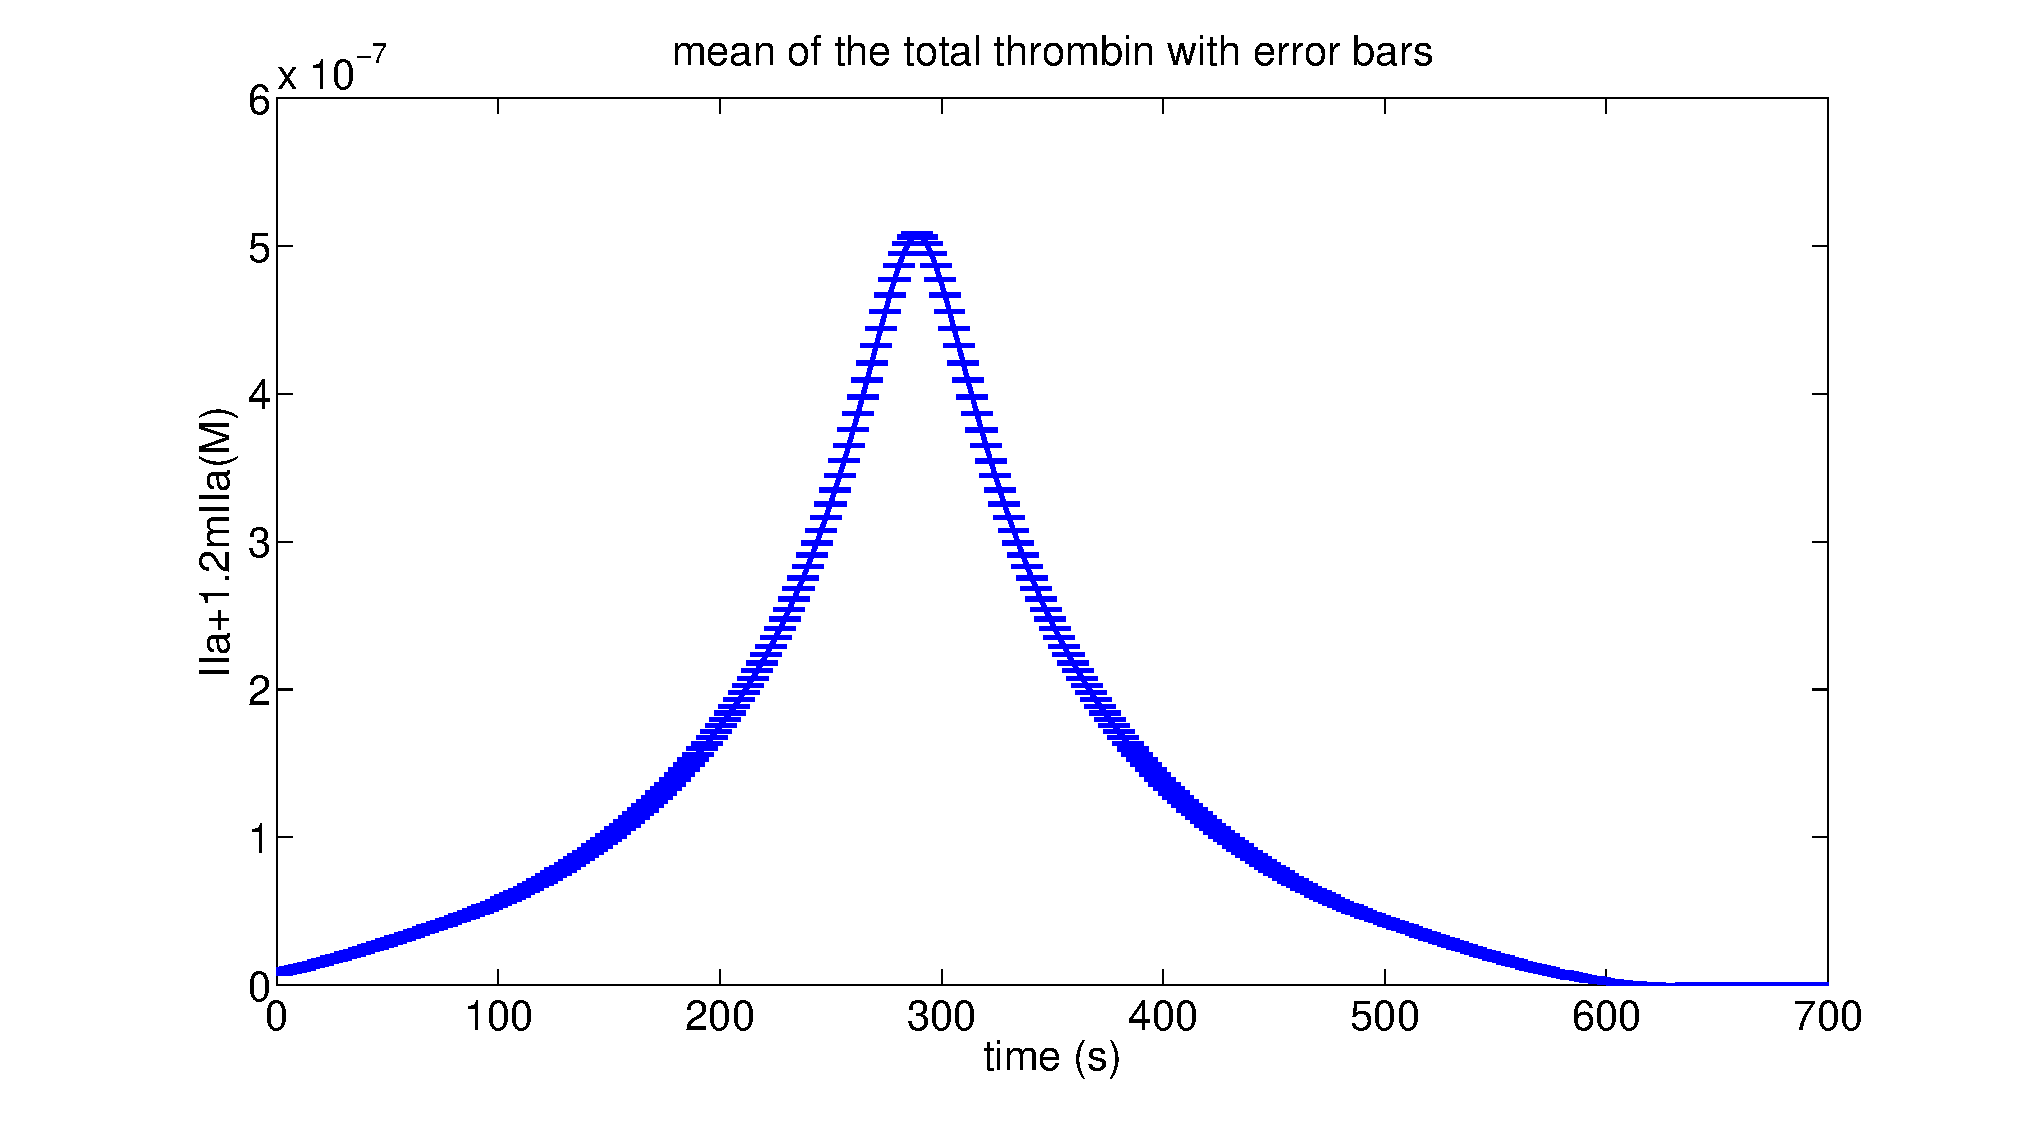
\includegraphics[width=5in]{figures/mean.eps}
\caption{The mean and error bar of the total thrombin along the
solution by time marching. Error bars show the confidence intervals
of reaction rates along the curve. }\label{Fig:mean}

  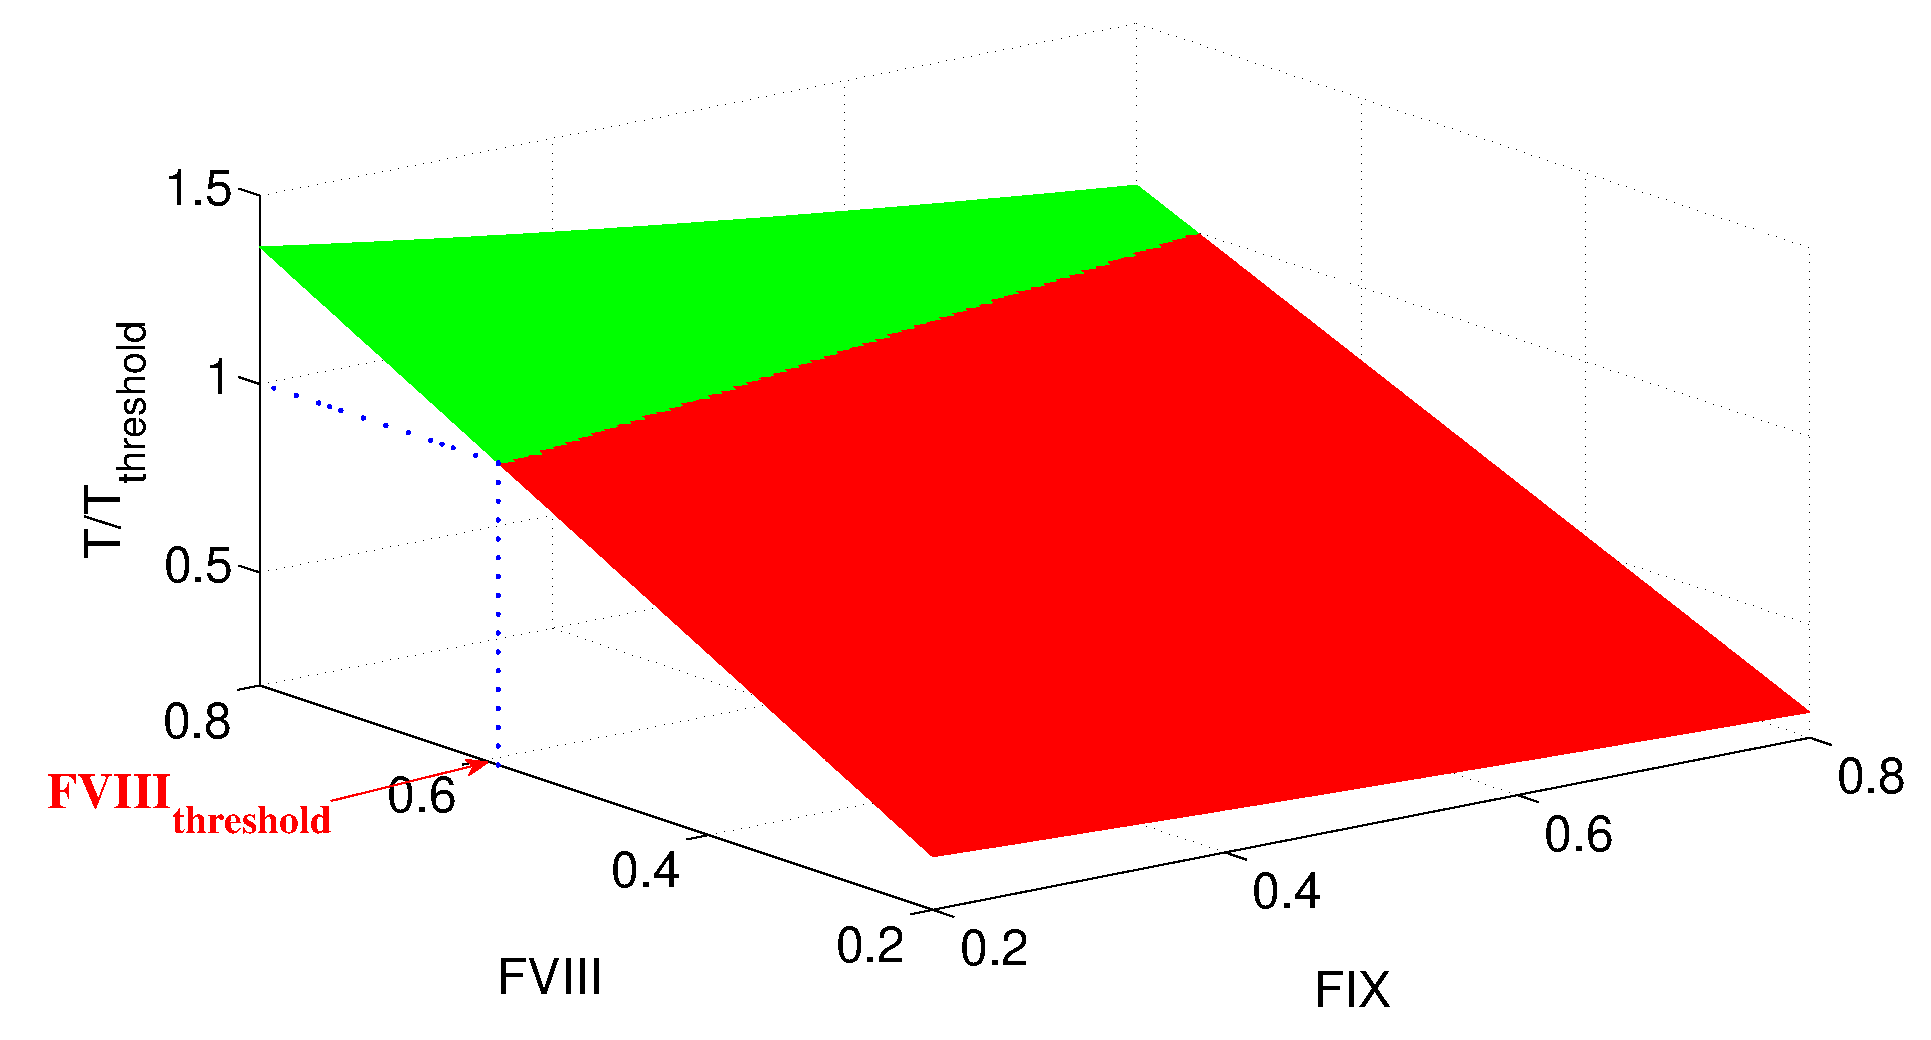
\includegraphics[width=5in]{figures/F89.eps}
\caption{The total thrombin \textit{v.s.} factors VIII (FVIII) and
IX (FIX). $T_{threshold}$ stands for the threshold  value of
thrombin. The red portion of the plane means the total thrombin (T)
is smaller than $T_{threshold}$ while the green portion means the
total thrombin is greater than $T_{threshold}$. This figure shows
that the threshold of factor VIII is 60 \% of normal value, and that
the total thrombin is greater than $T_{theshold}$ when factor VIII
is greater than $FVIII_{theshold}$ regardless of factor IX
concentration when it's in the assume range.}\label{Fig:F89}

  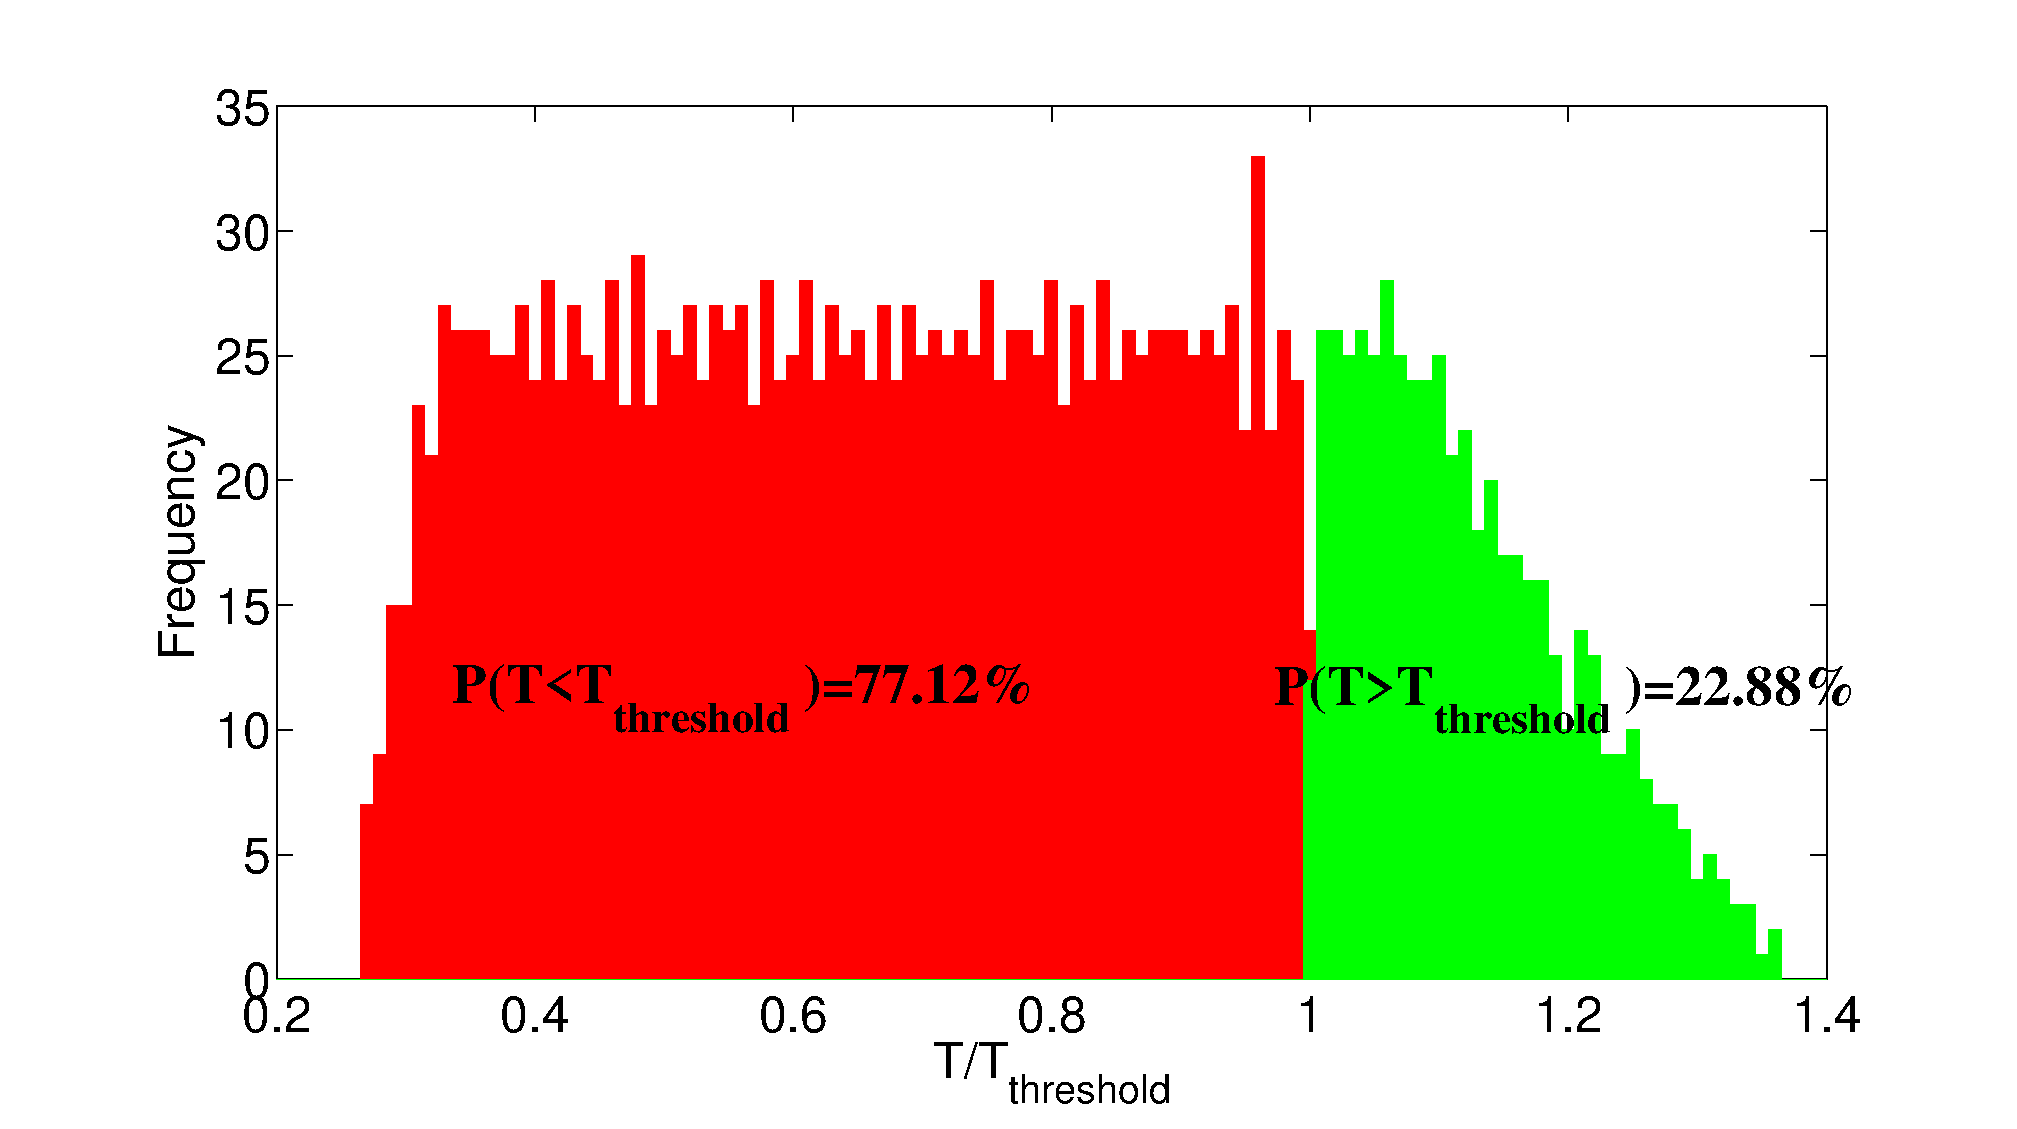
\includegraphics[width=5in]{figures/F89hist.eps}
\caption{Histogram of the total thrombin. The probability that the
total thrombin is greater than $T_{threshold}$ is
22.88\%.}\label{Fig:F89hist}

  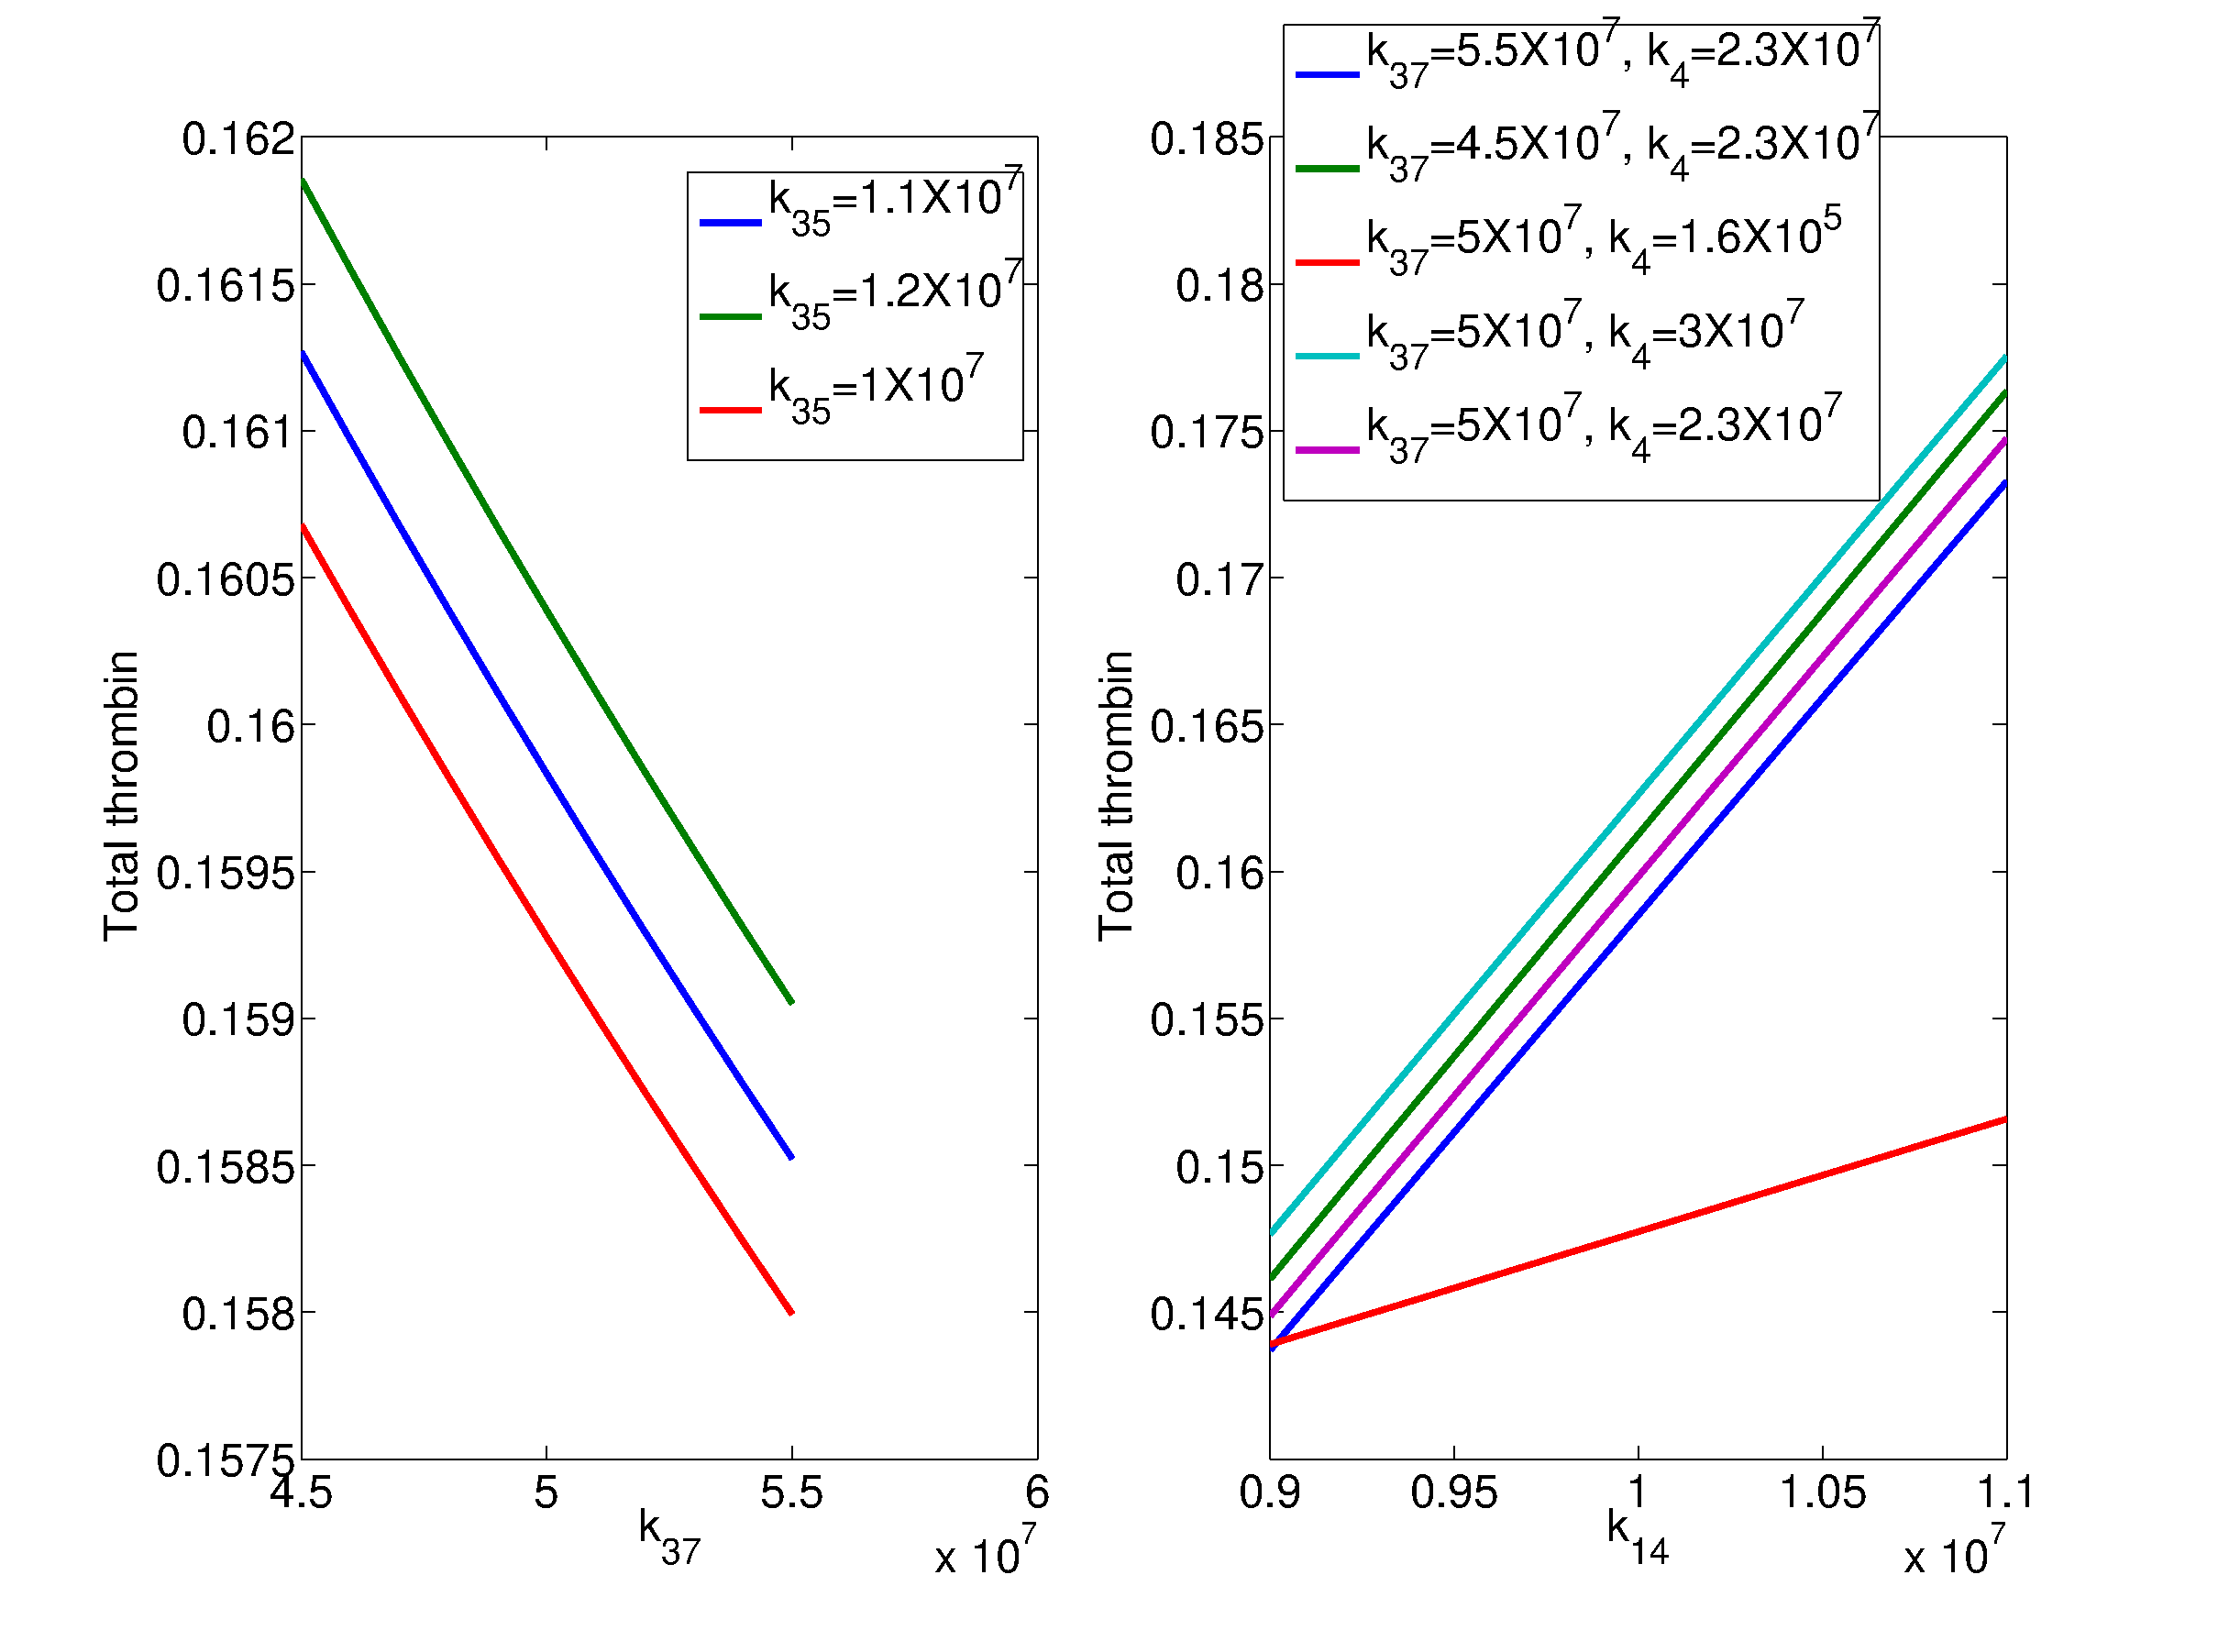
\includegraphics[width=5in,height=3in]{figures/rv.eps}
\caption{The total thrombin \textit{v.s.} reaction rates $k_{37}$
and $k_{14}$. $k_{37}$ inhibits the generation of total thrombin as
it increases. $k_{35}$ plays a negative role in the effect of
$k_{37}$. $k_{14}$ activates the generation of total thrombin as it
increases. $k_{37}$ and $k_4$ play negative and positive roles in
the effect of $k_{14}$ respectively.}\label{Fig:RV}

  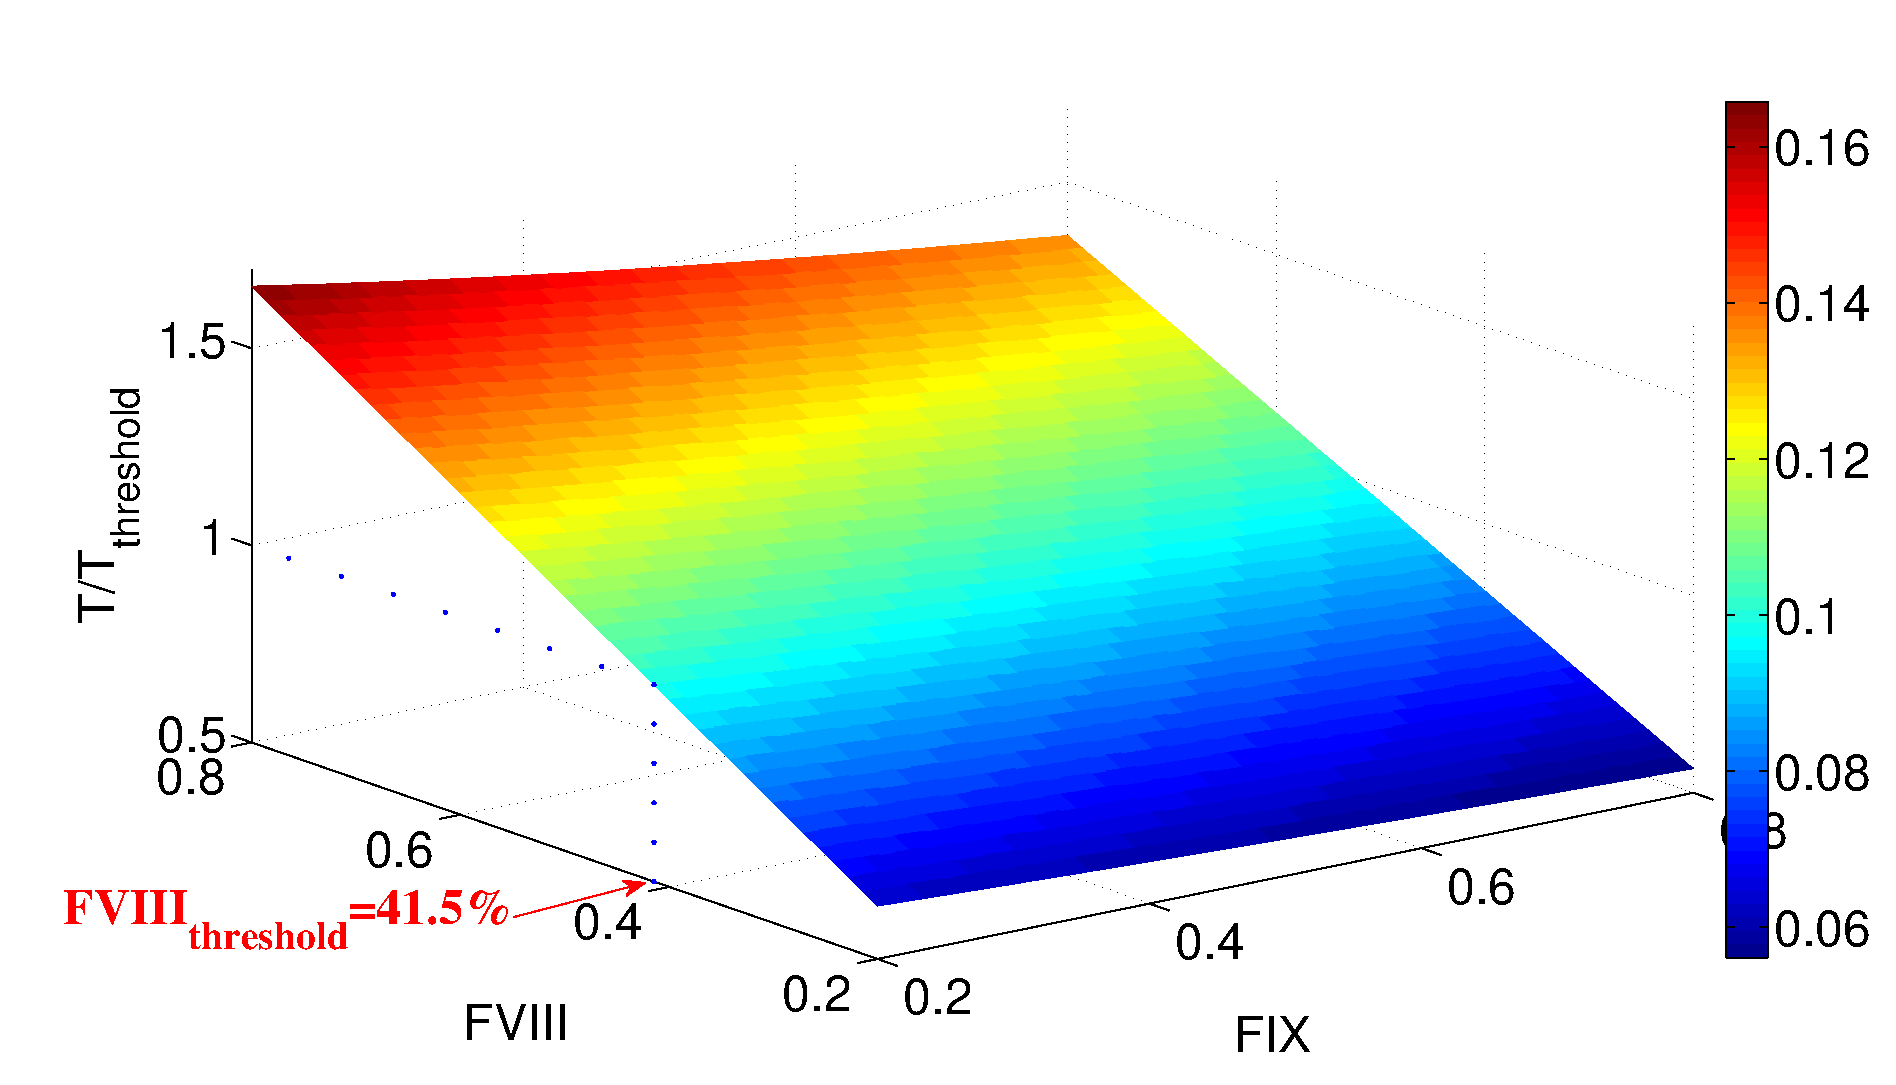
\includegraphics[width=5in]{figures/F89m.eps}
\caption{The mean of the total thrombin of sampling points of
$k_{14}$ and factor X, which vary from 100\%-200\% of their normal
values. The color means the variance of the total thrombin. This
figure shows that the threshold of factor VIII is decreased to 41.5
\% of normal value.}\label{Fig:F89m}

  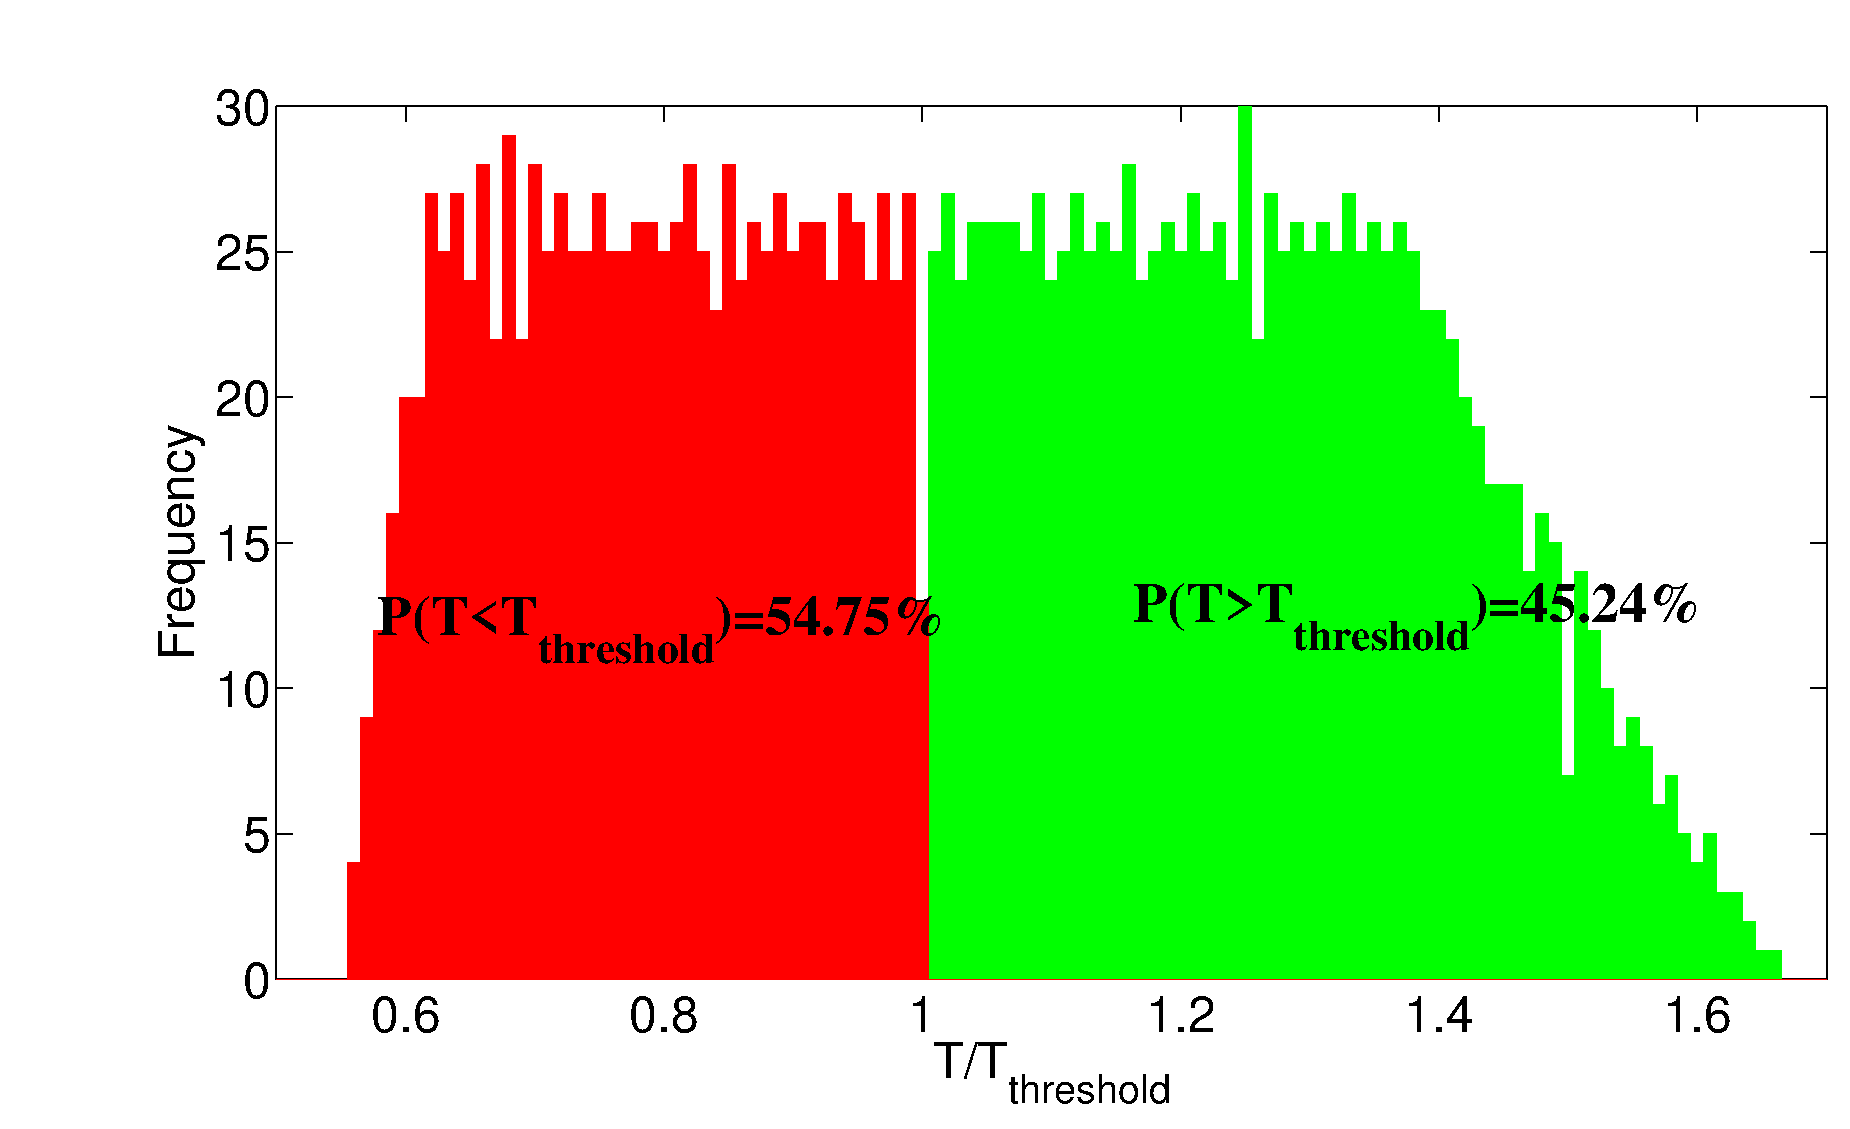
\includegraphics[width=5in]{figures/F89mhist.eps}
\caption{Histogram of the total thrombin as reaction rate $k_{14}$
and factor X is introduced. The probability that the total thrombin
is greater than $T_{threshold}$ is increased to
45.24\%.}\label{Fig:F89mhist}

  \includegraphics[width=5in,height=3.5in]{NSAD.eps}
\caption{ Network graph of importance of reaction rates and the
interaction between pair components with respect to total thrombin
when blocking $k_{14}$ and $k_{15}$ (their values are reduced by
90\%). See the legend in Figure 3. This figure shows that the
sensitivity shifts, i.e., reaction rate $k_{23}$ becomes the most
sensitive reaction rates in activating thrombin when $k_{14}$ and
$k_{25}$ are blocked. Moreover, $k_{13}$ plays no roles since
chemical reaction with $k_{13}$ is combined with $k_{14}$ and
$k_{25}$. }\label{Fig:NSAD}

  \end{center}
\end{figure}
